\chapter{Neural Network: Particle ID on imaging} \label{sec:NN_img}
Neural network and machine learning algorithm are powerful and versatile instruments that can improve the process of data analysis learning from datasets and making prediction with a certain degree of accuracy. Modern science, including physics, is taking more and more advantage of these techniques as the years go by.
The availability of big data is a key aspect in performing these studies and experimental particle physics is an area that can provide large datasets.\\

The chapter describes a possible application of deep neural networks on data generated through the IDEA DR Calorimeter full simulation with the aim to obtain simple particle identification analyzing the spatial deposited energy distribution.\\
An introduction to the computational techniques is provided, briefly describing the role of each component and the common structures that are used to perform the study.\\

All the data have to be prepared to be used in a neural network structure, the section \ref{sec:NN_data} shows which information has been used and how it has been processed to be analyzed by the deep learning algorithms.
After that the structures are presented in details showing the performances obtained in training and testing phases.\\
Eventually the study has been performed extending the energy range, the impact of this generalization conclude the chapter.\\
\newpage

\section{Project goal}
The chapter will explore the possibility to perform particle identification through neural network algorithms. The chosen task is to recognise and distinguish neutral pions and photons analyzing the spatial released energy distribution in a fixed area where the particles are fired.\\
As already introduced in paragraph \ref{subsec:em_shower}, photons produce electromagnetic showers in their path through matter. Considering the geometry of our DR calorimeter where the fibres are oriented towards the interaction point, a photon will release most of its energy in few adjacent fibres and the remnant energy will be absorbed by the surrounding fibres in a elliptical shape (an example can be seen in figure \ref{fig:demo_ph}.
On the other hand, the meson has a different behaviour. It decays in two main modes shown in figure \ref{fig:pi_decays}:
\begin{equation}
    \pi^0\xrightarrow{} 2\gamma \qquad \pi^0\xrightarrow{} \gamma + e^- + e^+
\end{equation}
The two decay mode have very different occurrence probability, in particular the $2\gamma$ decay has a branching ratio of $(98.823\pm0.034)\%$, instead it is $(1.174\pm0.035)\%$ for the gamma-electron-positron decay \cite{pi_decay}.\\
The consequence of this behaviour is that a electromagnetic shower is produced from each of the secondary particles. The result is a superposition of two or three (depending on which decay occurs) shower signals similar to the one produced by a single photon. In figure \ref{fig:demo_pi} the data obtained from a $\pi^0$ generation is sketched, it should be noted that, in the event represented, the meson decayed into two photons.\\

\begin{figure}
	\centering
	\subfloat[][$40\ GeV$ photon.\label{fig:demo_ph}]{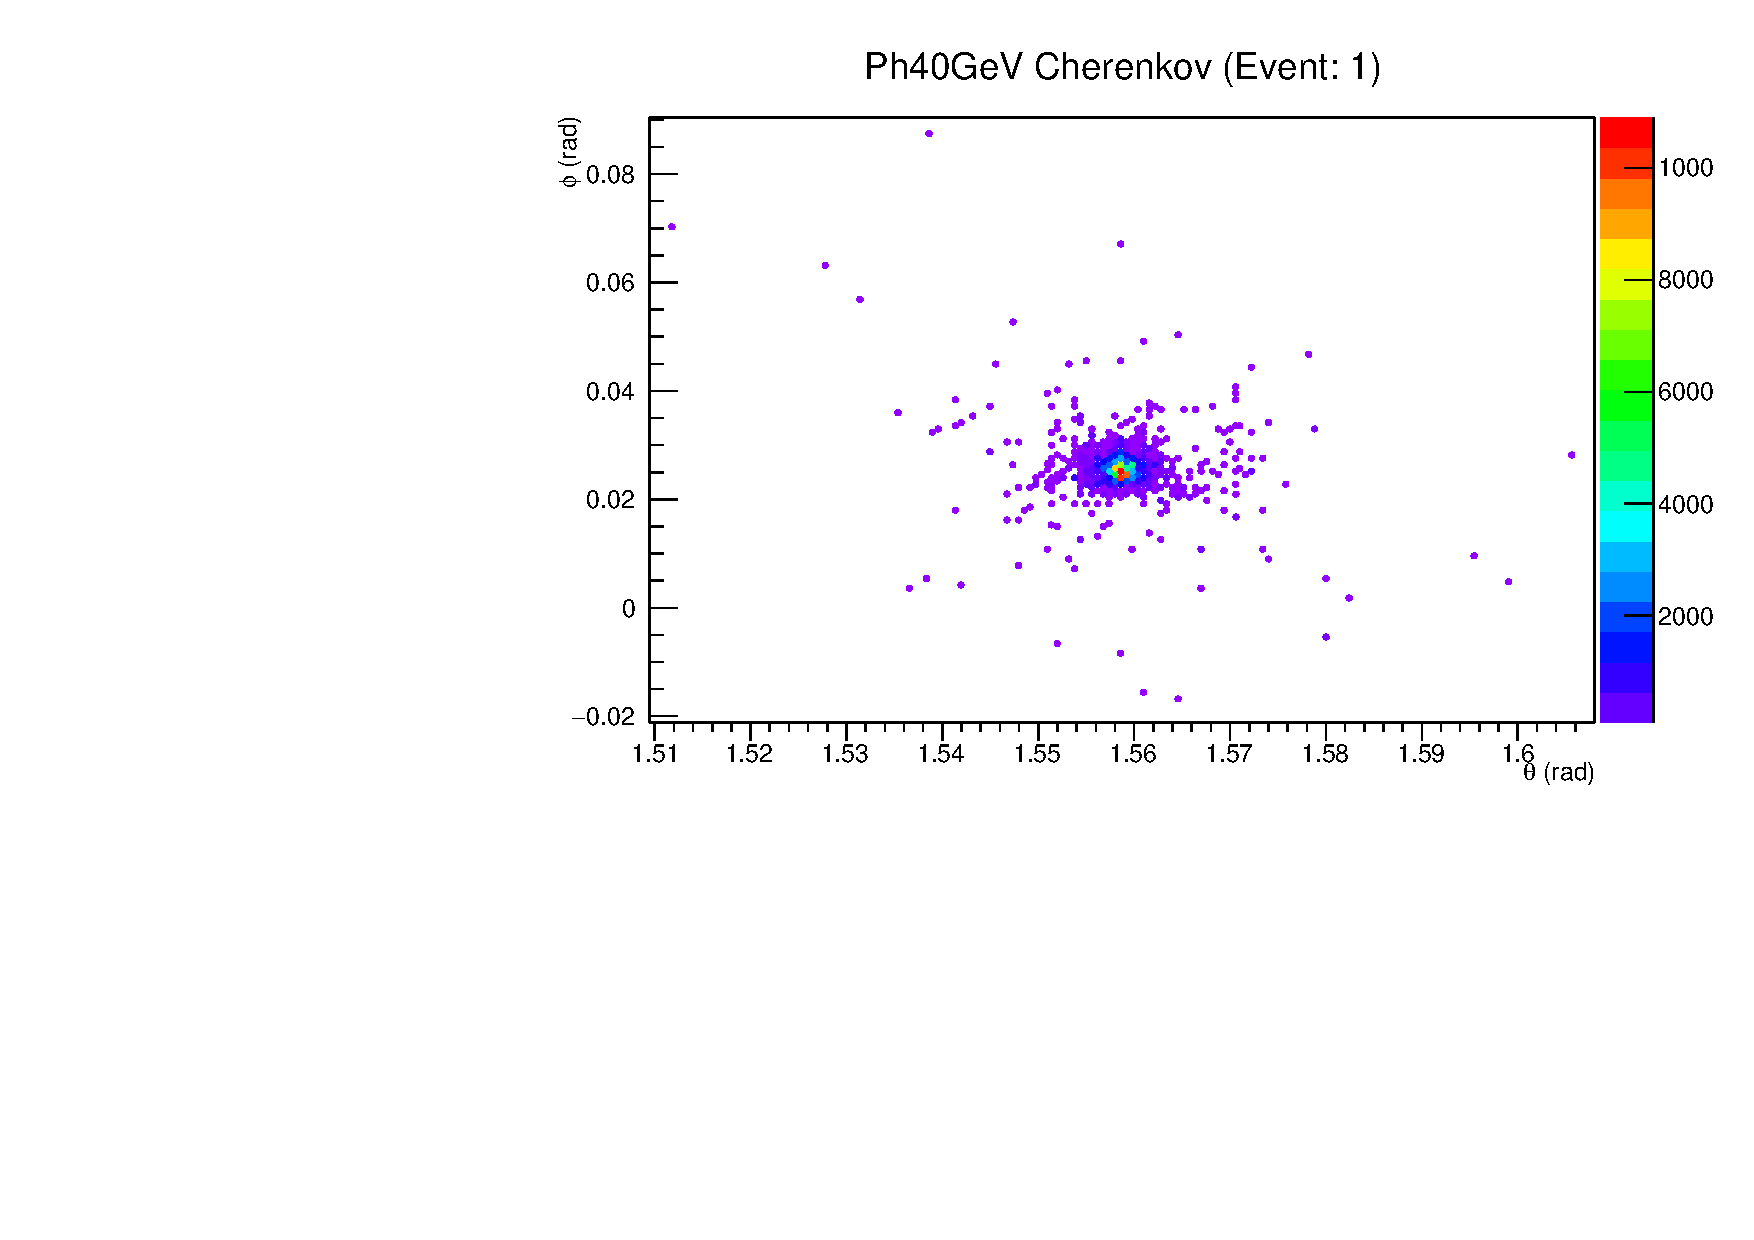
\includegraphics[width=.7\textwidth]{IMG/Cap6/Ph_01_cher.pdf}} \quad
	\subfloat[][$40\ GeV$ neutral pion.\label{fig:demo_pi}]{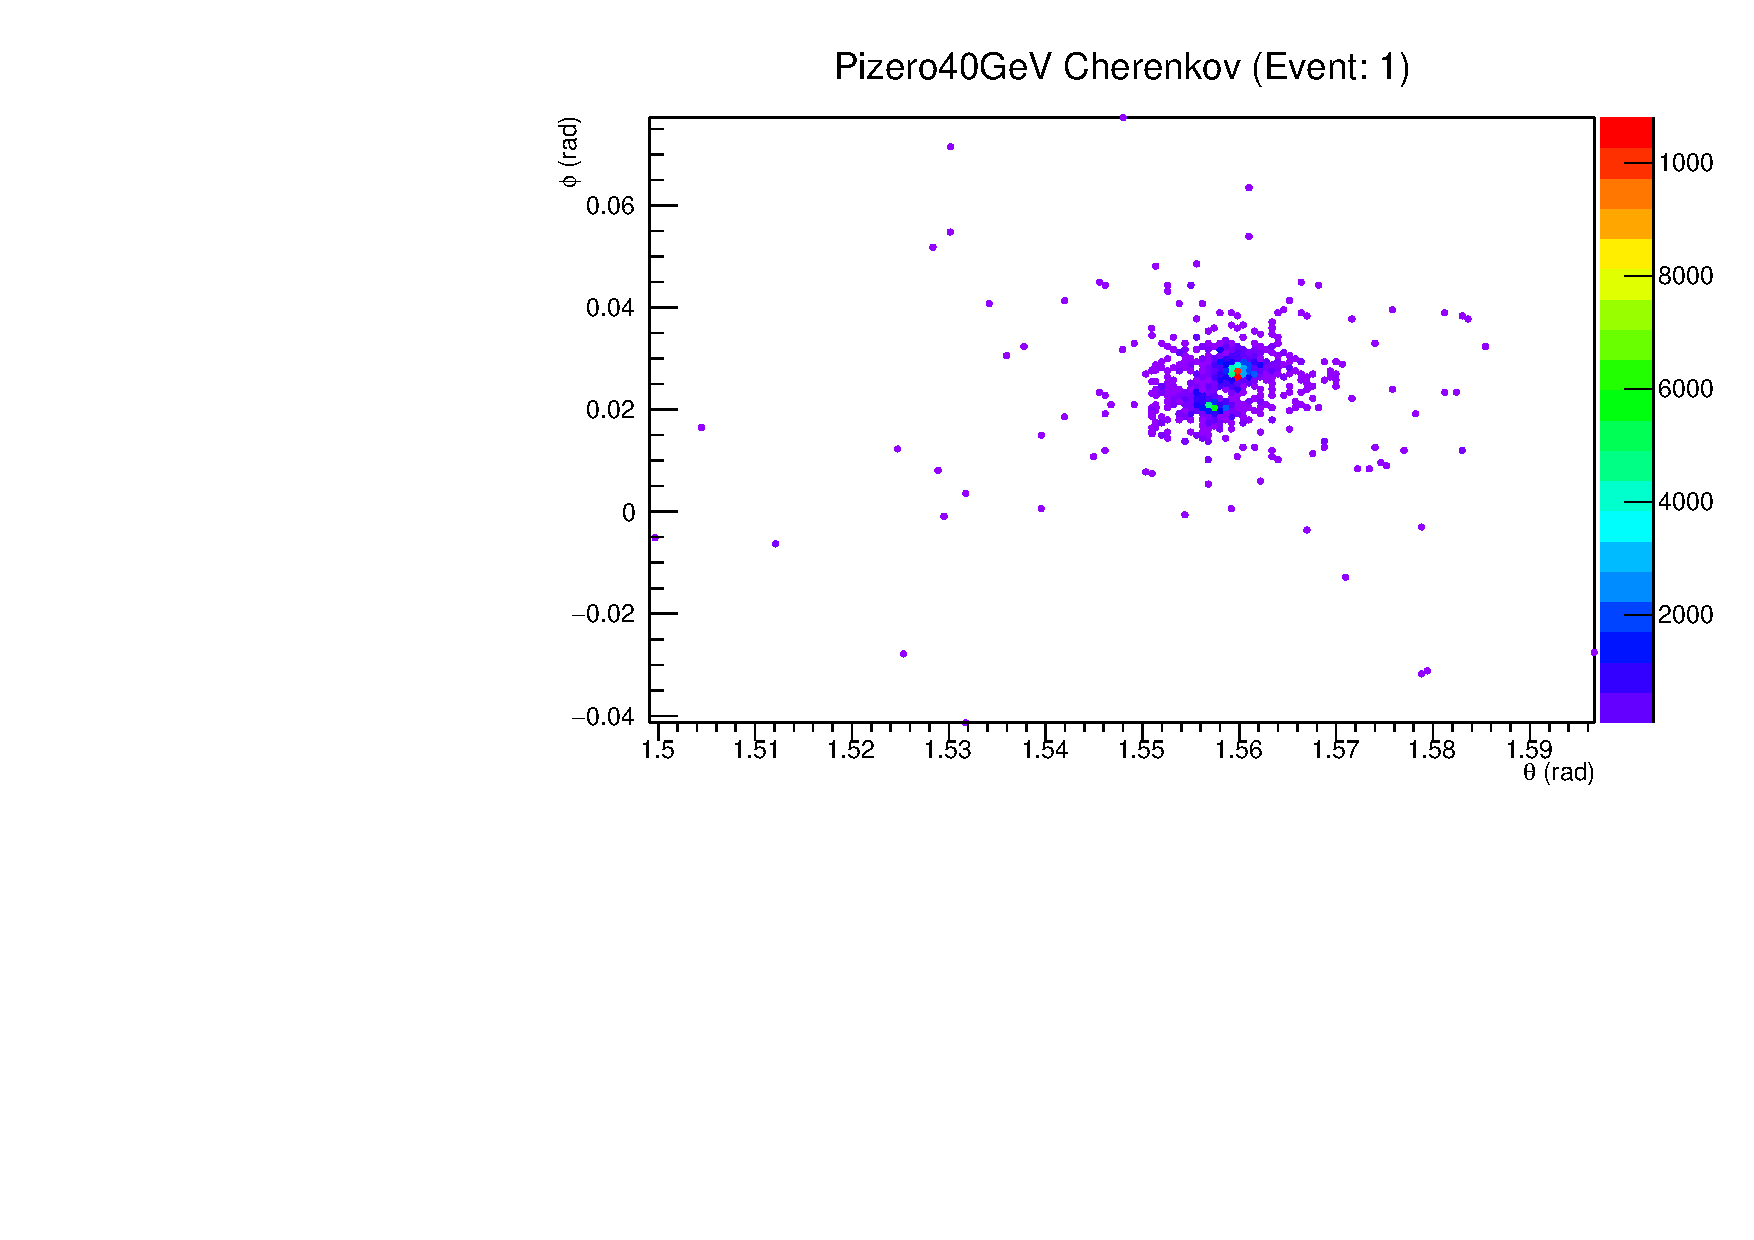
\includegraphics[width=.7\textwidth]{IMG/Cap6/Pizero_01_cher.pdf}}
	\caption{Spatial charge integral distributions from $\gamma$ and $\pi^0$. Each point correspond to an activated fibre and it is represented in cylindrical coordinates, the color indicates the charge integral obtained from the coupled SiPM.}
	\label{fig:demo_shower}
\end{figure}

\begin{figure}
	\centering
	\subfloat[][$\pi^0\xrightarrow{} 2\gamma$]{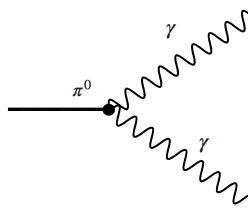
\includegraphics[height=.18\textheight]{IMG/Cap6/pi2gammas.png}} \quad
	\subfloat[][$\pi^0\xrightarrow{} \gamma + e^- + e^+$]{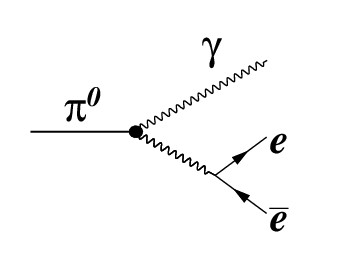
\includegraphics[height=.2\textheight]{IMG/Cap6/pi_gamma_e_e.jpg}}
	\caption{$\pi^0$ decay modes.}
	\label{fig:pi_decays}
\end{figure}

Usually this ID task would be performed applying a number of filters to study the elliptical shape, to find the peaks of charge integral, to measure the distances between the peaks and finally establishing, with a certain probability, the primary particle. The goal is to create a neural network able to accept data associated to an event and make a prediction on the primary particle with a small computational and timing effort.\\

\section{Neural Networks introduction}
Neural Networks are neural-inspired nonlinear models consisting in a group of artificial \textit{neurons} or \textit{nodes} interconnected through \textit{layers}. This type of architecture is supported by a mathematical structure where each neuron has an activation degree typically ranging from $0$ to $1$ and each edge is identified by weights and biases.\\

The simplest neural network structure follows a sequential model where neurons are grouped and linked to each other through \textit{layers} following a sequential order, but more complex neural networks implement also loops, branching and other different flows between layers.
The sequential model present a first input level followed by a series of hidden levels composed by hidden neurons and then connected to the output units. A visual representation is shown in figure \ref{fig:NN_art}.\\

\begin{figure}
	\centering
	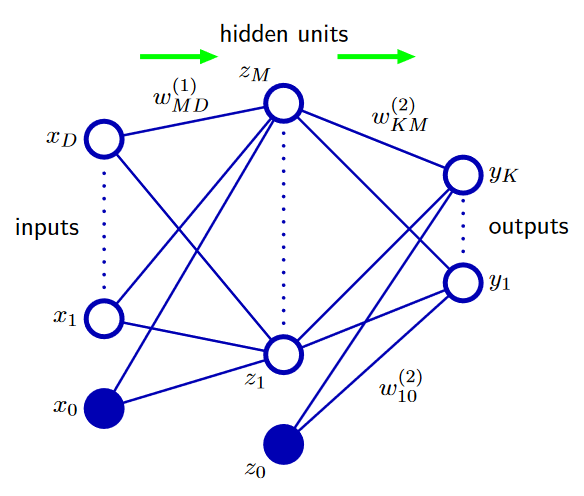
\includegraphics[width=.6\textwidth]{IMG/Cap6/NN_art.png}
	\caption{Schematic representation of a sequential model. The input, hidden, and output neurons are represented by nodes, and the weight parameters are represented by links between the nodes, for each connection the corresponding bias parameter is denoted by links coming from additional input and hidden variables $x_0$ and $z_0$. Green arrows indicate the direction of flow through the network. Figure from \cite{NN_Bishop}.}
	\label{fig:NN_art}
\end{figure}

The mathematical representation can be introduced studying a simple two-layer model. Starting from a D-dimension input vector $\bm{x}$, the first layer apply a linear combination for each hidden neuron in the next level:
\begin{equation}
    a_j^{(1)} = \sum_{i=1}^D w_{ij}^{(1)} x_i + w_{i0}^{(1)}
\end{equation}
where $j = 1,..., M$ (M is the layer output dimension) and the matrix $\bm{W}$ is the weights matrix including biases. The quantities $a_j$ are known as \textit{activations}. On these values a $h$ nonlinear function, called \textit{activation function}, is applied:
\begin{equation}
    z_j = h(a_j^{(1)})
\end{equation}
common activation function are \textit{sigmoid}, \textit{tanh}, \textit{ReLU} (rectified linear activation unit) and \textit{Softmax}. The obtained value are the already introduced hidden units and are used as input of the next layer. The process in the second layer is similar, valuating the following activations:
\begin{equation}
    a_k^{(2)} = \sum_{i=1}^M w_{jk}^{(2)} z_j + w_{k0}^{(2)}
\end{equation}
where $k = 1,..., K$ (K is the layer output dimension) and then applying the activation function. In the context of classification neural network, Softmax function ($S$) is a common choice of activation function in the last layer, providing the probability associated to each possible label.
\begin{equation}
    y_k = S(a_k^{(2)}).
\end{equation}
The whole process ca be represented in a single equation for each output neuron:
\begin{equation}
    y_k = S\left(\sum_{i=1}^M w_{jk}^{(2)} h\left(\sum_{i=1}^D w_{ij}^{(1)} x_i + w_{i0}^{(1)}\right) + w_{k0}^{(2)}\right).
\end{equation}
and, to obtain a more compact expression, the values $x_0=z_0=1$ can be introduced:
\begin{equation}
    y_k = S\left(\sum_{i=0}^M w_{jk}^{(2)} h\left(\sum_{i=0}^D w_{ij}^{(1)} x_i \right) \right)
\end{equation}
making even more clear the two-layer mathematical structure.\\

Once the neural network is set up a training process has to be performed to make the prediction consistent. In order to do that a large dataset of correctly labelled input has to be provided. During the training, the elements in the weight matrix $\bm{W}$ are constantly modified to adapt the output to be as closer as possible to the correct label. These are not random corrections but they are conditioned by a error function that quantifies the discrepancy between the output and the correct result. In classification tasks, a common error function choice is the \textit{cross-entropy} (given by the negative log likehood):
\begin{equation}
    E(\bm{w}) = -\sum_{n=1}^N\sum_{k=1}^K t_{nk}\ln{y_{nk}(\bm{x}_n,\bm{w})}
\end{equation}
where $t_n$ are the target vectors and $y_n=(\bm{x}_n,\bm{w})$ are the output vectors, with a dataset dimension of $N$ and $K$ different and mutually exclusive label possibilities.\\
The training aim is to correct the weights and biases values minimizing this error function.\\
Once this step is completed the neural network is ready to perform predictions and classify new data.\\

The study is performed with two different neural network structures that take advantages of few types of layers that will be briefly described.

\subsection*{Dense layer}
The dense layer is the simplest and most common layer, but far from being the lightest. It is classified as a fully connected layer, meaning that each output neuron receive an input value from each input node.\\
Mathematically, this type of layer consist in a matrix application on the input vector ($\bm{v}_i$) providing an output vector ($\bm{v}_o$), adding a bias vector ($\bm{w}_0$):
\begin{equation}
    \bm{v}_o = \bm{W}\bm{v}_i+\bm{w}_0.
\end{equation}

The layer is extremely parameter consuming, let consider a single layer that connects two group of nodes: it is common to use number of neuron that are powers of $2$ ($32$, $64$, $128$...). So the number of parameters associated to a single dense layer with an input dimension of $64$ and an output dimension of $32$ is:
\begin{equation*}
    64 \cdot 32 \text{(weights)} + 1 \cdot 32 \text{(biases)} = 2080
\end{equation*}
this number can increase very rapidly with the number of neurons.\\
Being the basic type of layer is often used to graphically represent general neural networks, figure \ref{fig:NN_art} shows sequence made by two consecutive dense layers.


\subsection*{Dropout layer}
Considering the extremely large number of training parameters, it is common practice to introduce the so called \textit{regularization} techniques to increase the capability of the neural network in generalizing well on new data. The use of a Dropout layer is one of them.\\
The basic idea is to reduce the spurious correlations that could occur between neurons in the network, preventing the overfitting. In practical terms, the dropout layer randomly "drops out" neurons (and the corresponding connections) following a probability $p$. This process is applied in each training step. An intuitive representation is sketched in figure \ref{fig:Drop}.

\begin{figure}
	\centering
	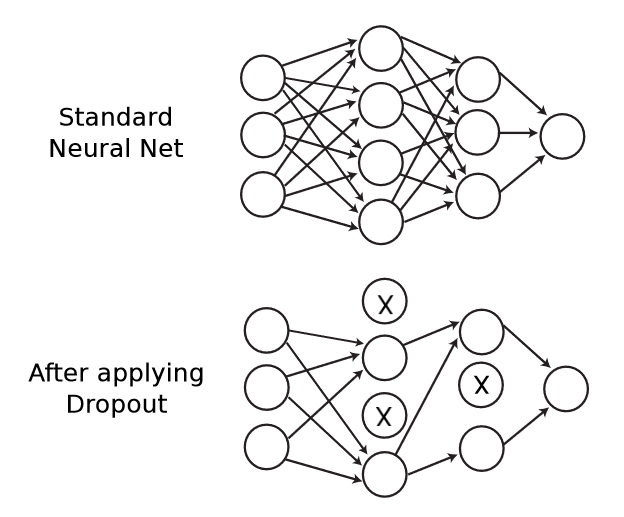
\includegraphics[width=.6\textwidth]{IMG/Cap6/Dropout.png}
	\caption{Neurons during training are randomly switched off with a probability $p$. A lighter network is produced reducing correlations between nodes. Figure from \cite{ML4ph}.}
	\label{fig:Drop}
\end{figure}

\subsection*{Conv2D layer}
A mandatory layer in analyzing images is the convolution layer and it identify a category of NN called Convolutional Neural Networks (CNNs).\\
A convolution consist in a simple application of a filter to an input that results in an activation. The application of the same filter repeatedly to the same input results in a map of activations called a feature map, this indicate the locations of a detected feature (and its intensity) in an input, such as an image.\\
Figure \ref{fig:Conv2D} represents the application of a filter or kernel ($K$) over a input matrix ($I$). As can be seen, the feature map is composed considering all the sub-images with the same size of the kernel, each sub-image is associated to an activation value obtained through the formula:
\begin{equation}
    a = \sum_{i = 1}^{D_K}\sum_{j = 1}^{D_K} I_{i,j} \cdot K_{i,j} + b
\end{equation}
where $D_K$ is the dimension of the kernel, typical values are $1$, $3$, $5$, and $b$ is the bias value. An activation is obtained from each sub-image and than corrected by the activation function, these outputs compose the feature map.\\
The layer output is a group of feature maps obtained from different filters. The number of filters evaluated represents the capability of the layer to identify different patterns.\\

In terms of trainable parameters, a convolution layer with $32$ kernels of $3\times3$ size is lighter then a dense one:
\begin{equation*}
    9\cdot 32 \text{(weights)} + 1 \cdot 32 \text{(biases)} = 320.
\end{equation*}

\begin{figure}
	\centering
	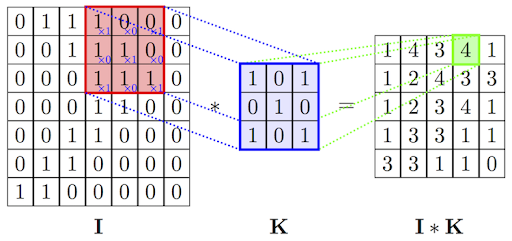
\includegraphics[width=.6\textwidth]{IMG/Cap6/ConvScheme.png}
	\caption{Example of convolution applying a single kernel $K$ on the input matrix $I$. The red square is the sub-image considered and convoluted with the blue matrix giving the activation value in the green box. The procedure is done over all the sub-images producing the feature map on the far right.}
	\label{fig:Conv2D}
\end{figure}

\subsection*{MaxPool2D layer}
A natural next-step to the convolution layer is represented by the category of pooling layers. This type of layers has the aim of reducing the size of the activation maps.\\
In particular, MaxPool2D layer consider a sub-matrix with a fixed size, typical $2\times2$ or $3\times3$, and record the max value. Performing the process over all the input matrix, the result is a smaller output matrix that keeps the geometrical feature information. A pictorial representation of the layer is shown in figure \ref{fig:MaxPool}.

\begin{figure}[b]
	\centering
	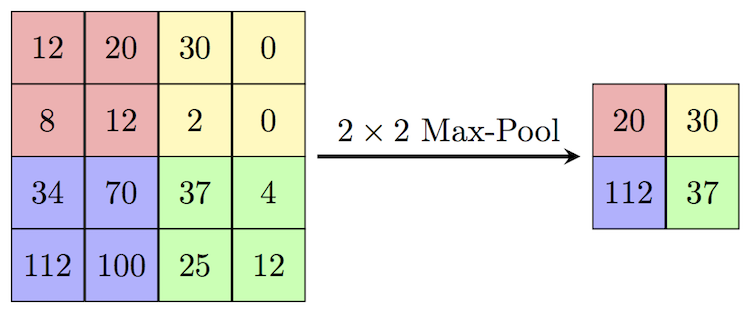
\includegraphics[width=.6\textwidth]{IMG/Cap6/MaxpoolSample2.png}
	\caption{MaxPool2D effect sketched where the same color represent the sub-matrix considered and the corresponding output.}
	\label{fig:MaxPool}
\end{figure}

%\subsection*{GlobalAveragePooling2D layer}


\subsection*{VGGNet structure}
The VGGNet structure is a neural network concept introduced in 2015 with the article "Very Deep Convolutional Networks for Large-Scale Image Recognition" \cite{VGGArt} (the name VGG is the acronym for Visual Geometry Group, their lab in Oxford).\\
The proposed, and then accepted as a standard, powerful structure is composed by several small-size filter chain (i.e. kernel size of $1\times1$ or $3\times3$), max pooling with size of $2\times2$ is used after most, but not all, the convolutional layers. The idea is that consecutive small-size filters approximate larger filter effects with an higher number of parameters. Another important characteristic is the large number of filters used: typically deeper layer has greater number of kernels starting from, at least, $32$.\\
In figure \ref{fig:VGG_table} the structure studied in \cite{VGGArt} are listed where groups of two or three convolutional layers are followed by max pooling ones, at the end the last max pooling layer output is flatten and used as input for a group of dense layers till the classification.\\

\begin{figure}
	\centering
	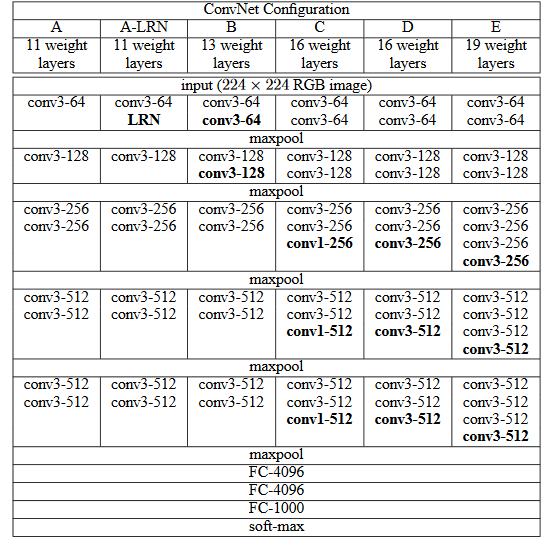
\includegraphics[width=.8\textwidth]{IMG/Cap6/VGG_art.png}
	\caption{Schematic representation of CNN structures studied by Karen Simonyan and Andrew Zisserman. Each column correspond to a CNN with different depth increasing from the left (A) to the right (E), as more layers are added (the added layers are shown in bold. The convolutional layer parameters are denoted as “conv[receptive field size]-[number of channels]".}
	\label{fig:VGG_table}
\end{figure}

A VGGNet like structure has been used to perform the task already introduced and it will be described in detail later (see paragraph \ref{sec:NN_perf}).

\subsection*{ResNet structure}
Residual Networks, or ResNet, are another innovative concept of CNN introduced in 2016 with the article "Deep Residual Learning for Image Recognition" by Kaiming He et al. \cite{ResNetArt}.\\
The structure is composed as a plain convolutional network with small kernel size (same as in VGGNet), this sequence of Conv-layers is splitted in several \textit{residual} blocks. The innovative aspect is that the input of each block is the sum of the input and the output of the previous block. The structure and flow of data are shown in figure \ref{fig:ResNet_scheme}, where two different ResBlock are sketched.\\

\begin{figure}
	\centering
	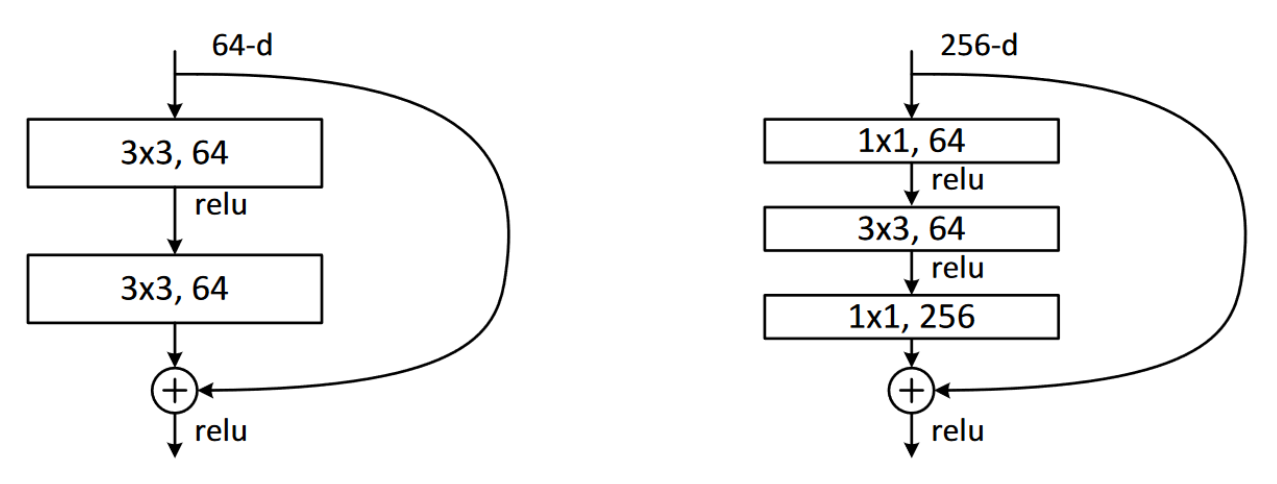
\includegraphics[width=.7\textwidth]{IMG/Cap6/ResNet_scheme.png}
	\caption{Schematic representation of residual blocks with arrows to indicate the data flow. On the left a simple two convolution block, on the right a "bottleneck" building block. Figure from \cite{ResNetArt}.}
	\label{fig:ResNet_scheme}
\end{figure}

The last block is followed by an average pooling layer (similar to the max pooling layer, but it record the average value and not the max value) and then a structure of consecutive dense layer till the classification one with softmax as activation function.\\

A ResNet like structure has been used to perform the task already introduced and it will be described in detail later (see paragraph \ref{sec:NN_perf}).

\section{Data setup}\label{sec:NN_data}
The data are produced through the IDEA DR Calorimeter full simulation, neutral pions and photons are fired from the interaction point to a fixed area of the calorimeter. In the first step particles with the fixed energy of $40\ GeV$ are produced.\\
Useful data from the simulation are:
\begin{itemize}
    \item starting fibre spatial coordinates ($x$, $y$, $z$);
    \item fibre type (Cherenkov or scintillating);
    \item charge integral from the SiPM digitization software.
\end{itemize}
The typical coordinate system for a $4\pi$ calorimeter is the spherical one so the cartesian coordinates have been transformed in spherical ones. Then, at each point the charge integral has been associated. Finally the are grouped in two subset by filtering with respect to the fibre types. The results obtained can be plotted in a 3D-graph to check the effective correctness of the process, an event taken as example can be seen in figure \ref{fig:3Dgraph}.

\begin{figure}
	\centering
	\subfloat[][Cherenkov signal.]{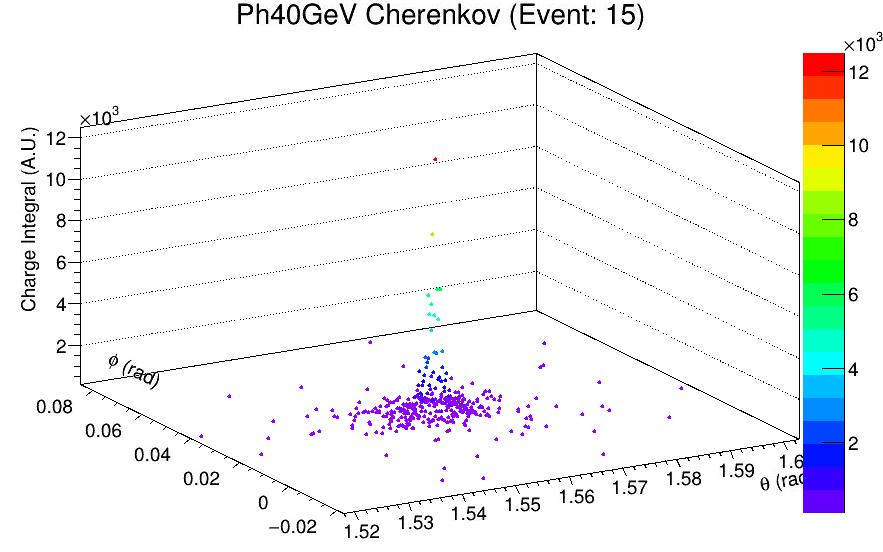
\includegraphics[width=.45\textwidth]{IMG/Cap6/ph40GeV_3Dgraph_cher.png}} \quad
	\subfloat[][Scintillation signal.]{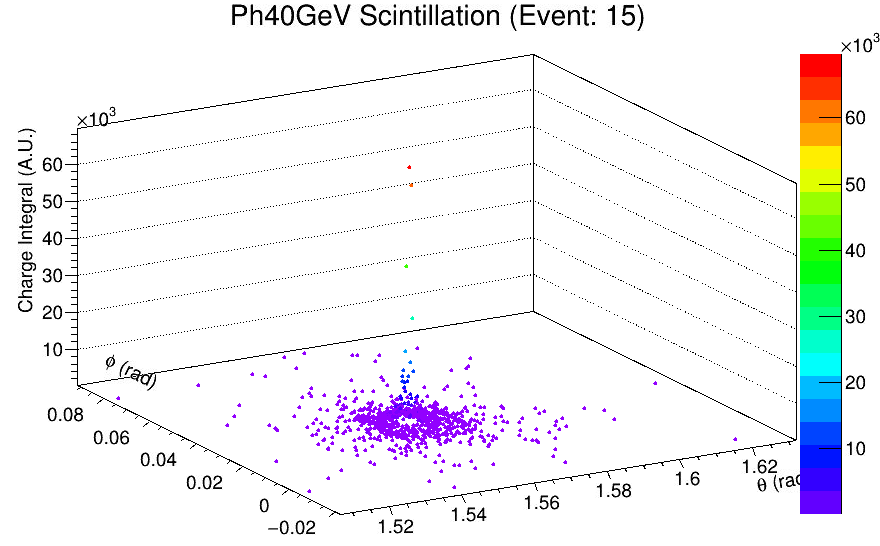
\includegraphics[width=.45\textwidth]{IMG/Cap6/ph40GeV_3Dgraph_scin.png}}
	\caption{3D-graphs representing Cherenkov and scintillation signals from the same sample event ($40\ GeV$ photon as primary particle).}
	\label{fig:3Dgraph}
\end{figure}

To train and take advantage of CNNs, the dataset has to be prepared. The input for VGGNet and ResNet has to be a dimension-fixed matrix for each event. Every event will be characterized by two features (Cherenkov charge integral and scintillation charge integral), each one of this represented by a grid reproducing the spatial distribution of the data. The squared area of interest in the $\theta-\phi$ space has been identified as $[(1.51,-0.02),(1.63,0.10)]$. Different values of grid step in this area has been compared reaching a good compromise between grid shape efficiency and imaging resolution choosing a grid step of $0.0009$ rad for both axes. The grid can be represented as 2D-histograms using the sum of all the charge integral values in each bin as bin height (figure \ref{fig:2Dhist} shows the histograms obtained from the same data in figure \ref{fig:3Dgraph}).\\
Hence the input matrix for each event has a shape of $133 \text{ (height) }\times 133\text{ (width) }\times 2\text{ (features)}$. A 2D visualization can be seen in figure \ref{fig:2Dvision}.\\

\begin{figure}
	\centering
	\subfloat[][Cherenkov signal.]{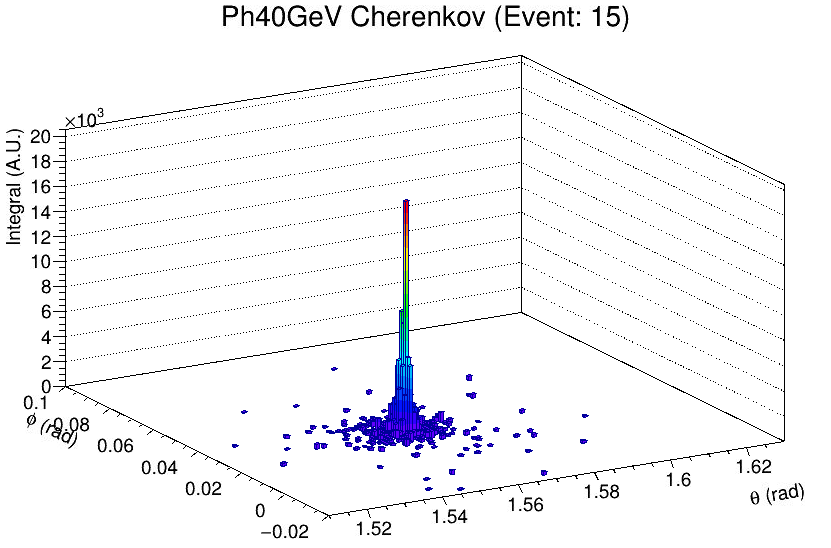
\includegraphics[width=.45\textwidth]{IMG/Cap6/ph40GeV_2Dhist_cher.png}} \quad
	\subfloat[][Scintillation signal.]{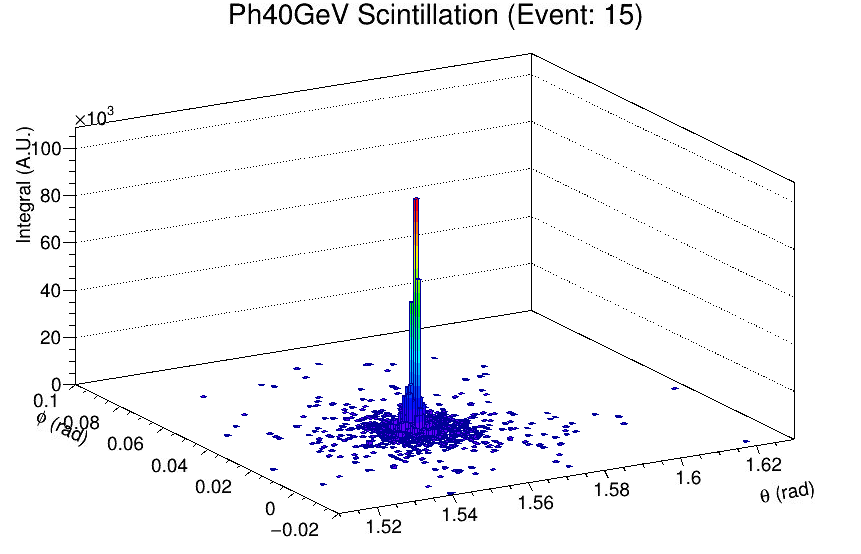
\includegraphics[width=.45\textwidth]{IMG/Cap6/ph40GeV_2Dhist_scin.png}}
	\caption{2D-histograms representing Cherenkov and scintillation signals from the same sample event ($40\ GeV$ photon as primary particle).}
	\label{fig:2Dhist}
\end{figure}

\begin{figure}
	\centering
	\subfloat[][Cherenkov signal pre data setup.]{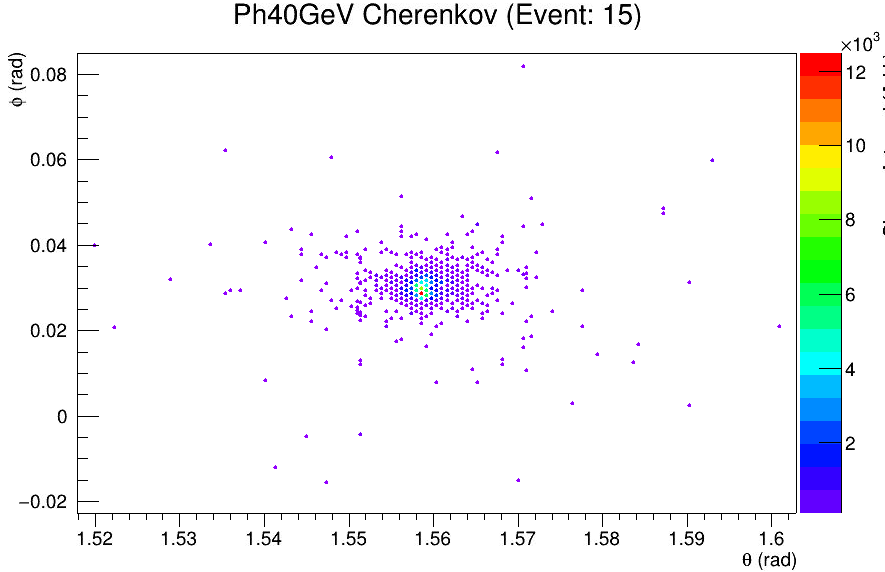
\includegraphics[width=.45\textwidth]{IMG/Cap6/ph40GeV_2Dvis_pre_cher.png}} \quad
	\subfloat[][Scintillation signal pre data setup.]{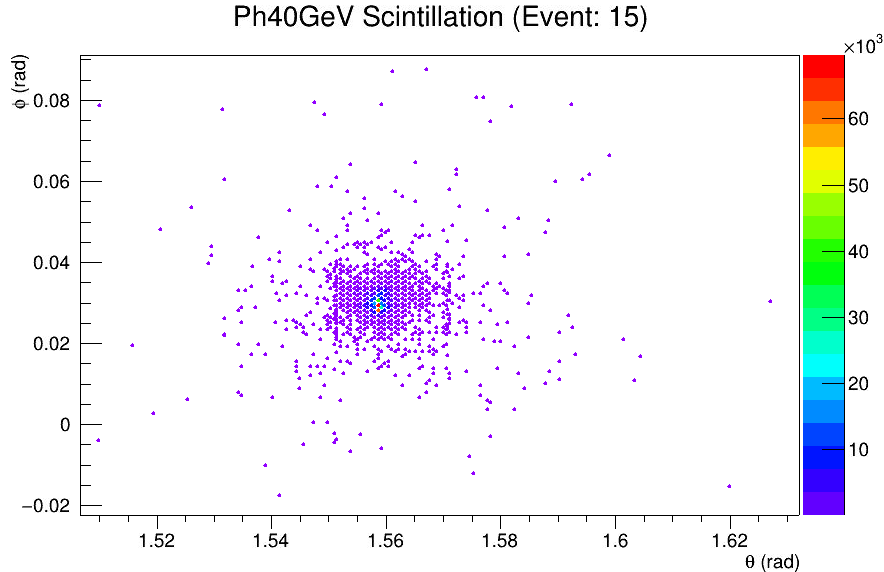
\includegraphics[width=.45\textwidth]{IMG/Cap6/ph40GeV_2Dvis_pre_scin.png}} \\
	\subfloat[][Cherenkov signal post data setup.]{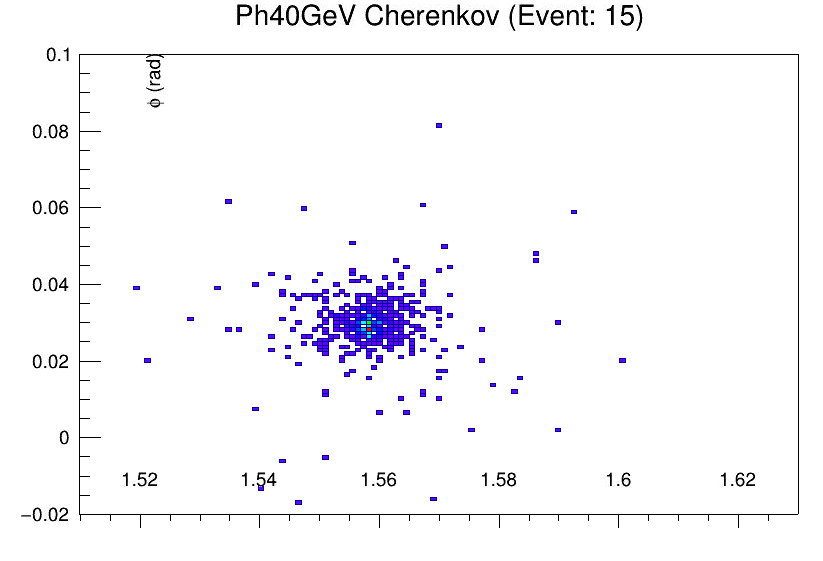
\includegraphics[width=.45\textwidth]{IMG/Cap6/ph40GeV_2Dvis_post_cher.png}} \quad
	\subfloat[][Scintillation signal post data setup.]{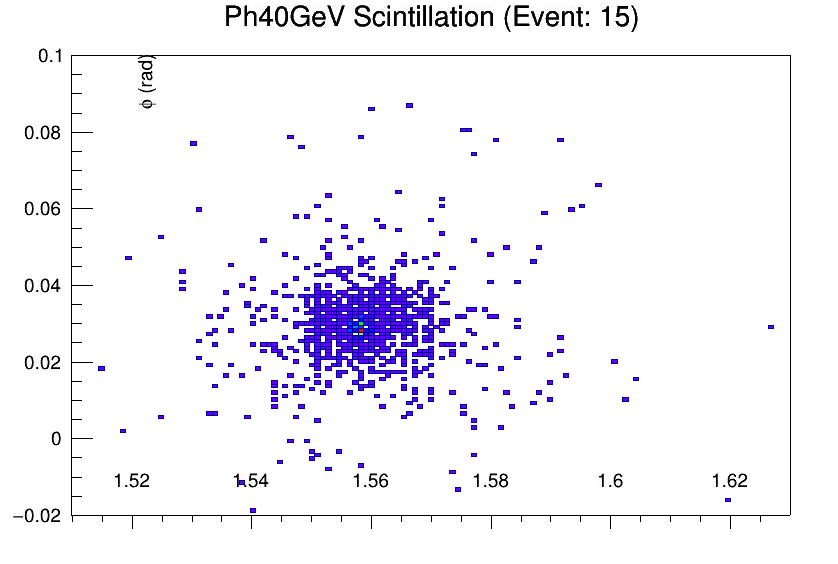
\includegraphics[width=.45\textwidth]{IMG/Cap6/ph40GeV_2Dvis_post_scin.png}}
	\caption{2D-vision of data before and after data setup.}
	\label{fig:2Dvision}
\end{figure}

The complete process of data preparation is applied on $10000$ events of photons and $10000$ events of neutral pions. All the events have been labelled ($\gamma$ and $\pi^0$), normalized to the max value of $1$ (same normalization constant for all the dataset), shuffled and splitted in two sub-set dedicated to training ($80\%$) and to validation ($20\%$).\\

\section{Performances}\label{sec:NN_perf}
aaa

\section{Energy range extension}
aaa